\section{Bộ nhớ chính}

Để lưu trữ dữ liệu, một máy tính chứa một tập các mạch (kiểu như Flip-Flops), mỗi mạch có
khả năng lưu trữ một bít. Dãy bít này gọi là \textbf{bộ nhớ chính} của máy.

\subsection*{Tổ chức bộ nhớ}
Bộ nhớ chính của máy tính được tổ chức theo các đơn vị dễ quản lý, gọi là các \textbf{ô
  nhớ}, một ô nhớ thường gồm tám bít (hay là một \textbf{byte}). Với các máy tính nhỏ dùng
cho các thiết bị gia đình như lò vi sóng, bộ nhớ chính của nó có thể chỉ gồm vài nghìn ô
nhớ. Trong khi các máy tính lớn có thể có bộ nhớ chính lên tới hàng tỷ ô nhớ.

Các ô nhớ trong máy tính không có thứ tự. Tuy nhiên, ta vẫn thường quy ước sắp xếp chúng
theo hàng. Phía phải nhất của hàng này được gọi là ở vị trí \textbf{cao} và phía trái được
gọi là vị trí \textbf{thấp}. Mỗi vị trí (byte) của hàng ta lại đánh thứ tự tính từ
\textit{phải qua trái}. Bít phía trái nhất có trọng số cao nhất và cũng thường được gọi là
\textbf{bít dấu} (cách gọi này dựa theo cách biểu diễn giá trị số của ô nhớ.).  Ta có thể
biểu diễn nội dung của ô nhớ với kích thước tính theo byte như theo Hình~\ref{fig:fig1.8}.

\begin{figure}[tb]
\centering
    \scalebox{0.4}{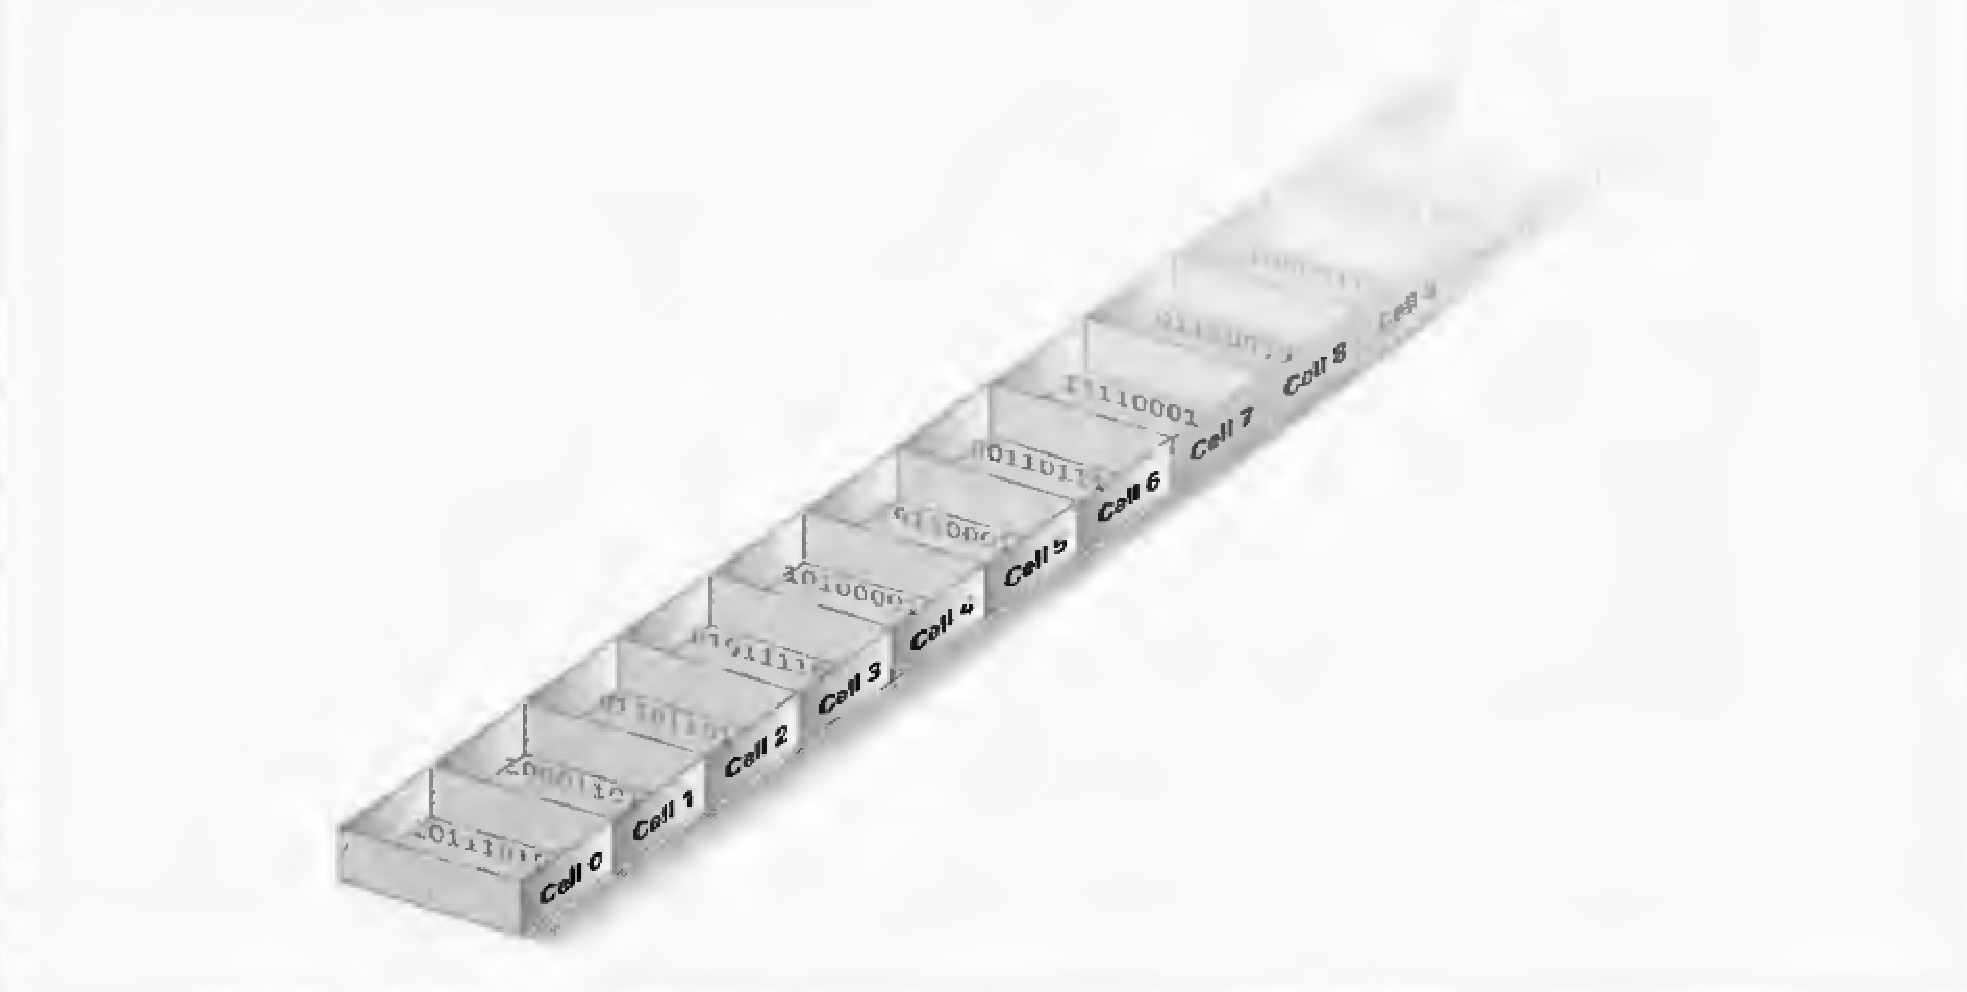
\includegraphics{ch2/Fig1-8.pdf}}
\caption{Các ô nhớ được sắp xếp theo địa chỉ}
  \label{fig:fig1.8}
\end{figure}

Để xác định ô nhớ trong bộ nhớ chính, mỗi ô nhớ được gán với một ``tên'' duy nhất, được
gọi là \textbf{địa chỉ}. Phương pháp này tương tự với cách đánh địa chỉ nhà trong thành
phố. Chính xác hơn, ta nhìn các ô nhớ xếp theo hàng và đánh số bắt đầu từ $0$. Cách đánh
địa chỉ kiểu này cho ta cách xác định ô nhớ một cách duy nhất. Tuy vậy, nó cũng gắn cho
các ô nhớ một thứ tự (Hình \ref{fig:fig1.8}), thứ tự này cho phép ta sử dụng các thuật ngữ ``ô
nhớ tiếp theo''  hoặc thuật ngữ ``ô nhớ trước''.


Việc gán thứ tự cho các ô nhớ trong bộ nhớ chính và các bít bên trong mỗi ô nhớ cho phép
ta đánh thứ tự các bít của  bộ nhớ chính theo hàng. Vậy ta có thể lưu trữ các
dãy bít có kích thước lớn hơn kích thước  của một ô nhớ. Ví dụ, ta có thể lưu trữ các xâu $16$ bít bằng hai ô nhớ liên tiếp.

% Để bổ trợ cho bộ nhớ chính, các mạch thực sự lưu trữ các bít được tổ
% hợp với mạch được yêu cầu để cho phép mạch lưu trữ và lấy dữ liệu từ
% các ô nhớ. Theo cách này, các mạch khác có thể lấy dữ liệu từ bộ nhớ
% bằng cách hỏi nội dung của một số ô nhớ (được gọi là thao tác đọc bộ
% nhớ), hoặc chúng có thể ghi thông tin vào trong bộ nhớ bằng cách yêu
% cầu một số bít đặt trong ô nhớ tại địa chỉ đặc biệt (được gọi là phép
% toán ghi).
%[.....]

Bởi vì bộ nhớ chính của máy tính được tổ chức như tập các ô nhớ riêng biệt được địa chỉ
hoá, nên các ô nhớ này có thể được truy cập một cách độc lập theo yêu cầu (cách truy cập
này của bộ nhớ chính ngược lại với cách truy cập của thiết bị lưu trữ khối, là thiết bị
trong đó các xâu bít dài được xử lý theo từng  khối). Để mô tả khả năng có thể
truy nhập được vào mọi ô nhớ, bộ nhớ chính được gọi là \textbf{bộ nhớ truy cập ngẫu nhiên
  (RAM)}.

Ta đã giới thiệu các Flip-Flop để lưu trữ các bít, nhưng trên thực tế bộ nhớ RAM trong
các máy tính hiện đại thường được xây dựng theo kỹ thuật khác. Kỹ thuật này cho phép bộ
nhớ có kích thước nhỏ hơn và có thời gian trả lời nhanh hơn. Thông thường, người ta dùng các  mạch điện nhỏ dễ  bị mất điện tích để lưu trữ các bít. Bởi vậy các thiết
bị này thường cần thêm các mạch, gọi là mạch làm tươi, chịu trách nhiệm nạp điện nhiều
lần một giây.

Để đoán nhận việc hay thay đổi này, bộ nhớ máy tính được xây dựng từ kiểu kỹ thuật này gọi là
bộ nhớ động, dẫn tới thuật ngữ \textbf{DRAM} (Dynamic RAM). Hoặc, tại thời điểm viết quyển
sách này, người ta hay nói tới \textbf{SDRAM} (Synchronous DRAM, có nghĩa rằng DRAM có sử
dụng kỹ thuật đồng bộ (Synchronous) làm giảm thời gian cần thiết để lấy nội dung của một ô
nhớ.)

\subsection*{Đơn vị đo khả năng bộ nhớ}
Ta sẽ thấy trong chương tiếp theo rằng việc thiết kế hệ thống bộ nhớ chính trong đó tổng
số ô nhớ là một luỹ thừa của $2$ có rất nhiều điểm tiện lợi. Kích thước của bộ nhớ trước
đây thường được tính theo $1024$ (bằng $2^{10}$) đơn vị ô nhớ. Bởi vì $1024$ là gần với
giá trị $1000$, người ta thường sử dụng tiền tố \textit{kilo} cho đơn vị này. Có nghĩa
rằng, thuật ngữ \textit{kilobyte} (viết tắt là KB) được sử dụng để chỉ $1024$ byte. Bởi
vậy, một máy với $4096$ ô nhớ được gọi là có $4$KB bộ nhớ ($4096 = 4 \times 1024$). Khi bộ
nhớ trở nên lớn hơn, thuật ngữ này được phát triển thêm bao gồm các tiền tố \textit{mega}
cho $1,048,576$ (bằng $2^{20}$) và \textit{giga} cho $1,073,741,824$ (bằng $2^{30}$), và
đơn vị như MB (megabyte) và GB (gigabyte) trở nên phổ biến.

Không may, việc áp dụng các tiền tố thể hiện đơn vị tính có thể gây nhầm lẫn vì các tiền
tố này đã được sử dụng trong các lĩnh vực khác theo đơn vị đo là luỹ thừa của~$10$. Ví dụ,
khi tính khoảng cách, một \textit{kilo-mét} tương ứng bằng $1000$ mét, và khi đo tần xuất
radio, một \textit{mega-hertz} tương ứng bằng $1,000,000$ hertz. Tình huống còn tệ hơn khi
một số nhà sản xuất thiết bị máy tính còn pha trộn hai kiểu thuật ngữ này, dùng KB để
chỉ~$1024$ byte nhưng MB theo nghĩa là $1000$KB (bằng $1,024,000$ byte). Điều này gây lộn
xộn và không rõ ràng cho người dùng thuật ngữ này.

Để làm rõ ràng, người ta đề nghị dùng tiền tố \textit{kilo, mega}, và \textit{giga} cho
các đơn vị theo luỹ thừa của~$10$, và đưa thêm các tiền tố mới \textit{kibi} (viết tắt
kilobinary và ký hiệu là Ki), \textit{mebi} (viết tắt cho megabinary và ký hiệu là Mi), và
\textit{gibi} (viết tắt cho gigabinary và ký hiệu là Gi) tương ứng với đơn vị theo luỹ
thừa của $2$. Với hệ thống này, thuật ngữ \textit{kibibyte} (KiB) có thể để chỉ $1024$
byte, trong khi đó \textit{kilobyte} (KB) dùng để chỉ $1000$ byte. Các thuật ngữ này có
trở thành phổ biến hay không thì phải chờ thời gian trả lời. Hiện tại các thuật ngữ bị
hiểu nhầm \textit{kilo, mega,} và \textit{giga} vẫn bị ăn sâu trong cộng đồng người sử
dụng khi nói tới bộ nhớ chính, bởi vậy ta vẫn theo các ký hiệu truyền thống trong các
nghiên cứu khi tham khảo đến việc lưu trữ dữ liệu. Tuy vậy, các tiền tố \textit{kibi,
  megi}, và \textit{gibi} được đưa ra nhằm giải quyết vấn đề này, và có thể rằng là khôn
ngoan khi diễn dịch các thuật ngữ như \textit{kilobyte} và \textit{megabyte} kèm theo lời
cảnh báo.

\subsection*{Câu hỏi \& Bài tập}
\begin{enumerate}
\item Nếu ô nhớ số $5$ chứa giá trị $8$, hãy chỉ ra sự khác nhau giữa việc viết
  giá trị~$5$ vào ô nhớ số $6$ và chuyển nội dung của ô nhớ số $5$ vào ô nhớ số $6$?

\item Giả sử rằng bạn muốn hoán đổi các giá trị được lưu trữ tại ô nhớ số $2$ cho ô nhớ số
  $3$. Cách thực hiện sau đây có gì sai:
  \begin{description}
  \item \textit{Bước 1.} Chuyển nội dung của ô nhớ số $2$ vào ô nhớ số $3$.
  \item \textit{Bước 2.} Chuyển nội dung của ô nhớ số $3$ vào ô nhớ số $2$.
  \end{description}
  Thiết kế một dãy các bước thực hiện đúng việc tráo đổi nội dung của hai ô nhớ này.

\item Có thể lưu trữ bao nhiêu bít vào bộ nhớ máy tính có dung lượng $4$KB (chính xác hơn
  là KiB)?
  
\end{enumerate}
\section{Thiết bị lưu trữ khối}

Do tính không bền vững và kích thước hạn chế của bộ nhớ chính, nên hầu hết các máy tính
đều có thêm thiết bị nhớ,  gọi là các hệ thống lưu trữ khối (hoặc là lưu trữ thứ
cấp). Các thiết bị này bao gồm đĩa từ, CD, DVD, băng từ, và ổ đĩa flash (ta sẽ thảo luận
các thiết bị này sau). Ưu điểm của hệ thống lưu trữ khối so với bộ nhớ chính là tính lưu
trữ thông tin lâu dài, khả năng lưu trữ lớn, giá thành thấp, và trong nhiều trường hợp cho
ta khả năng có thiết bị lưu trữ tạm thời có thể tách rời khỏi máy.

Thuật ngữ \textit{on-line} và \textit{off-line} thường được sử dụng để mô tả thiết bị được
gắn hoặc tách rời khỏi máy. \textbf{On-line} có nghĩa rằng thiết bị hoặc thông tin được
kết nối và sẵn sàng để đọc từ máy mà không cần sự can thiệp của con
người. \textbf{Off-line} có nghĩa rằng cần sự can thiệp của con người trước khi thiết bị
hoặc thông tin có thể truy cập được từ máy--có thể bởi vì thiết bị phải được bật, hoặc cơ
cấu làm việc yêu cầu các thông tin trung gian phải được thêm vào.

Điểm bất lợi chính của thiết bị lưu trữ khối yêu cầu các dịch chuyển cơ học và bởi thế
chúng cần nhiều thời gian hơn để lưu trữ và nhận dữ liệu từ máy so với bộ nhớ chính, nơi
mà mọi hoạt động đều được thực hiện bằng điện.

\subsection*{Các hệ thống từ tính}


Theo thời gian, các công nghệ từ đang chiếm ưu thế trong lĩnh vực lưu trữ khối. Ví dụ, thiết bị  điển hình được  sử dụng ngày nay là \textbf{đĩa từ}, gồm các đĩa tròn được phủ từ được dùng để lưu trữ dữ liệu. Các đầu đọc/ghi được đặt ở trên và/hoặc dưới đĩa, và khi đĩa xoay tròn,
mỗi đầu đọc đi theo một vòng tròn, gọi là một \textbf{track}, quanh bề mặt bên trên và bên
dưới của đĩa. Bằng cách đặt lại vị trí của đầu đọc/ghi, ta có thể truy cập vào các track đồng tâm khác nhau. Trong nhiều trường hợp, hệ thống lưu trữ bao gồm một vài đĩa được gắn
với một ống suốt chung, đĩa này đặt trên đĩa khác, và khe nhỏ ở giữa hai đĩa đủ đặt các
đầu đọc/ghi. Các đầu đọc/ghi dịch chuyển theo cách thống nhất. Mỗi lần đầu đọc/ghi đặt
lại vị trí, ta lại có một tập mới các track, được gọi là \textbf{cylinder}, có thể truy
cập vào được.

Bởi vì một track thường chứa nhiều thông tin  hơn số thông tin ta muốn xử lý tại một thời điểm,
nên ta lại chia nhỏ mỗi track thành các cung, gọi là \textbf{sector}. Thông tin trên
các sector này được ghi như các xâu bít liên tục (Hình \ref{fig:fig1.9}). Các sector trên
một đĩa có thể có cùng số bít (thông thường là nằm trong khoảng từ $512$ byte tới một
KB). Trong trường hợp đơn giản nhất, hệ thống lưu trữ đĩa có số sector trên mỗi track là
bằng nhau. Vì các track bên ngoài có chu vi lớn hơn so với các track ở bên trong, nên
trong trường hợp này số bít trong một sector trên track ở phía ngoài của đĩa lưu trữ ít
dày đặc hơn so với các track ở gần trung tâm. Trên thực tế, với những hệ thống đĩa có khả
năng lưu trữ cao, các track ở phía ngoài xa trung tâm thường chứa nhiều sector hơn track ở
gần trung tâm. Ta có được khả năng này là nhờ áp dụng một kỹ thuật gọi là
\textbf{zoned-bit recording}. Dùng zone-bit recording, một vài track kề nhau được tập hợp
thành một vùng, các đĩa điển hình chứa khoảng mười vùng. Mọi track trong một vùng có cùng
số sector, nhưng các vùng bên ngoài có nhiều sector trên một track so với vùng bên trong
nó. Theo cách này, không gian lưu trữ của đĩa được sử dụng hiệu quả hơn so với cách của hệ
thống đĩa truyền thống. Nói một cách đơn giản, đây là một hệ thống lưu trữ bao gồm nhiều
sector riêng, mỗi sector có thể được truy cập như một xâu bít độc lập.

\begin{figure}[tb]
\centering
    \scalebox{0.3}{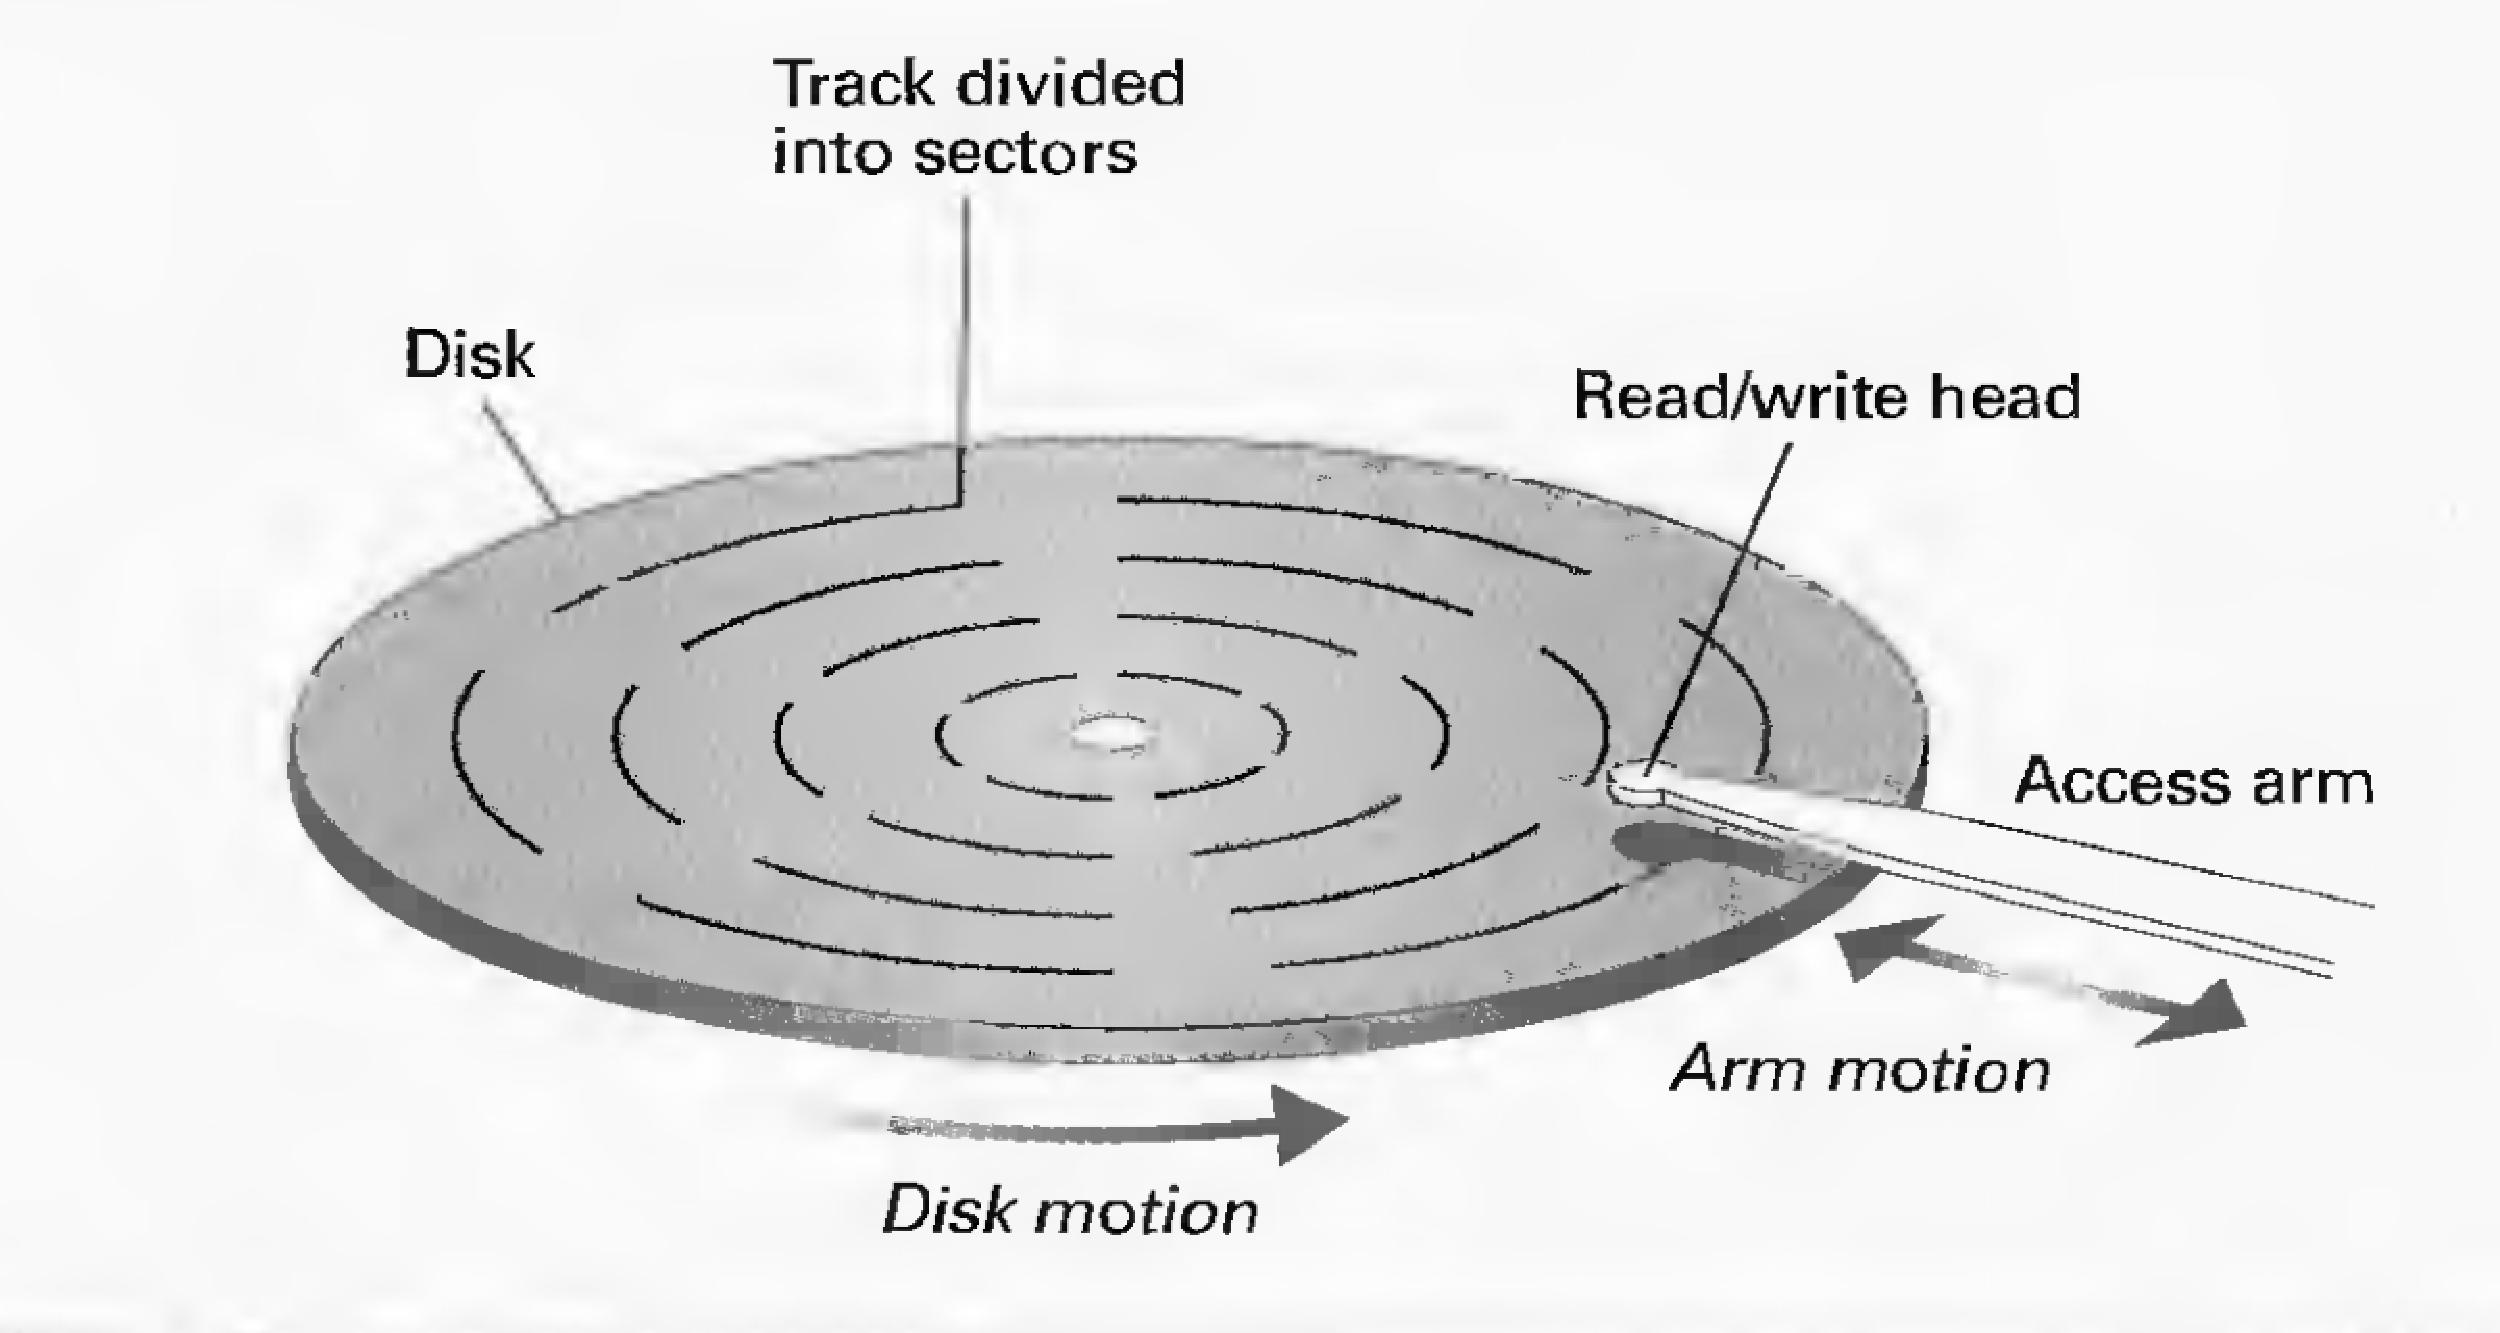
\includegraphics{ch2/Fig1-9.pdf}}
\caption{Một hệ thống lưu trữ đĩa}
  \label{fig:fig1.9}
\end{figure}

Vị trí các track và sector là có thể thay đổi so với cấu trúc vật lý
đĩa. Chúng được đánh dấu về mặt từ tính qua một quá trình gọi là \textbf{formating} (hay
khởi tạo) đĩa. Quá trình này thường được thực hiện bởi nhà sản xuất đĩa, kết quả ta được
một đĩa đã được format. Tuy vậy, hầu hết hệ thống máy tính đều có thể thực hiện nhiệm vụ
này. Bởi vậy, nếu thông tin format trên đĩa bị hỏng, đĩa có thể được format lại. Tuy nhiên
quá trình này sẽ phá huỷ mọi mọi thông tin đã được lưu trữ ghi trên đĩa trước đó.

Khả năng của hệ thống lưu trữ đĩa phụ thuộc vào số đĩa được sử dụng và mật độ track và
sector được thiết đặt. Các hệ thống mức thấp chỉ gồm một đĩa được làm bằng chất dẻo, gọi là \textbf{đĩa mềm}, hay bởi một tên ít dùng hơn là \textbf{floppy}. Đĩa mềm dễ đưa
vào và lấy ra từ các ổ đọc/ghi, đồng thời dễ được lưu trữ lại. Vậy nên đĩa mềm được
dùng rất phổ biến như thiết bị lưu trữ thông tin off-line. Tuy nhiên, bởi vì đĩa
mềm~$3\frac{1}{2}$-in chỉ có khả năng lưu trữ $1.44$MB, nên nó đã nhanh chóng
bị thay thế bởi công nghệ khác.

Các hệ thống đĩa có khả năng lưu trữ cao có thể lưu trữ lên tới nhiều gigabyte. Chúng có
thể bao gồm năm đến mười đĩa cứng đặt trên cùng một trục. Do các đĩa này được làm bằng
chất liệu cứng nên chúng thường được gọi là hệ thống đĩa cứng, ngược lại với thuật ngữ đĩa
mềm. Để cho phép tốc độ quay nhanh, các đầu đọc/ghi trong các hệ thống này không chạm vào
đĩa mà chỉ ``lơ lửng'' trên bề mặt đĩa. Không gian dành cho đầu đọc ở giữa hai đĩa là rất
hẹp, thậm chí chỉ một ít bụi cũng có thể làm kẹt đầu đọc và bề mặt đĩa, dẫn đến phá huỷ cả
hai (hiện tượng này gọi là vỡ đầu đọc). Bởi vậy nên các hệ thống đĩa cứng thường được đặt
bên trong case máy tính và được đóng kín bởi nhà sản xuất.

% Có một vài độ đo để đánh giá hiệu năng hệ thống đĩa:
% \begin{inparaenum}
% \item[(1)] \textbf{thời gian di chuyển} (thời gian chuyển đầu đọc từ track
%   này sang track khác).
% \item[(2)] \textbf{độ trễ vòng quay} hay \textbf{thời gian trễ}
% \end{inparaenum}

%[....]

Hệ thống đĩa cứng nói chung có những đặc trưng tốt hơn so với đĩa mềm. Bởi vì đầu đọc/ghi
không chạm vào bề mặt đĩa, nên nó có tốc độ quay lên tới vài nghìn vòng trong một
phút. Trong khí đó hệ thống đĩa mềm quay chỉ khoảng $300$ vòng một phút. Do đó tốc độ
truyền của hệ thống đĩa cứng, thường là vài MB trên giây, lớn hơn rất nhiều so với đĩa mềm
(chỉ vài KB trên giây).

Do các thao tác của hệ thống đĩa yêu cầu chuyển động về mặt vật lý, nên nó kém hơn rất
nhiều so với tốc độ của mạch điện tử. Thời gian trễ của mạch điện được tính theo đơn vị
nano giây (một phần tỷ của giây) hoặc ít hơn, trong khi đó thời gian di chuyển, thời gian
trễ và thời gian truy cập của hệ thống đĩa được tính theo mili-giây (một phần nghìn của
giây). Bởi vậy, khi các mạch điện đợi lấy kết quả từ hệ thống đĩa, thời gian dường như là
vô tận.

Không chỉ có hệ thống lưu trữ đĩa là thiết bị lưu trữ khối dùng công nghệ từ. Một dạng cũ
hơn của lưu trữ khối dùng công nghệ từ là \textbf{băng từ} (Hình \ref{fig:fig1.10}). Trong
các hệ thống này, thông tin được ghi dưới dạng một băng mềm mỏng quấn xung quanh một ống
để lưu trữ.
 
%[.....]

\begin{figure}[bth]
  \centering \scalebox{0.4}{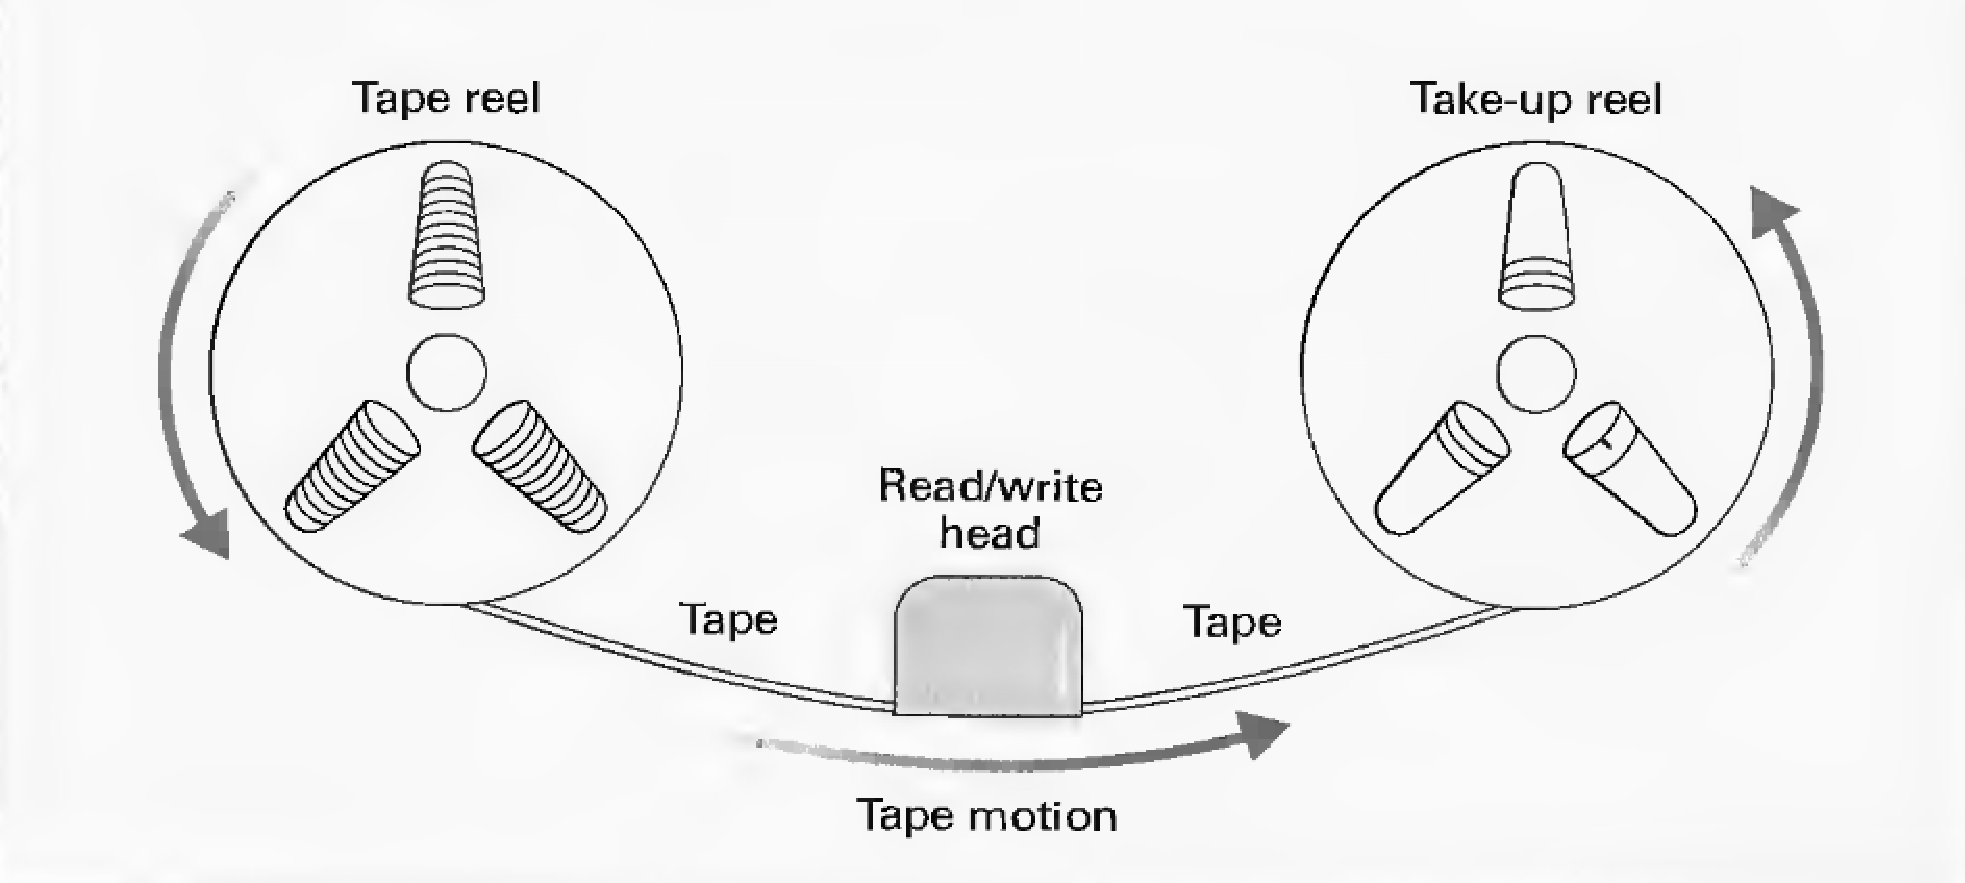
\includegraphics{ch2/Fig1-10.pdf}}
\caption{Cơ chế lưu trữ băng từ}
  \label{fig:fig1.10}
\end{figure}

\subsection*{Hệ thống quang}

Có một lớp thiết bị lưu trữ khối áp dụng kỹ thuật quang. Ví dụ đĩa \textbf{CD} (Compact
Disk). Các đĩa này có đường kính là $12$cm (xấp xỉ $5$ inches) và được phủ một lớp gương
với một lớp phủ bảo vệ. Thông tin được ghi trên đĩa bằng cách thay đổi bề mặt phản xạ. Vì
vậy, các thông tin này có thể được lưu trữ theo cách chùm tia laser được phóng không theo
quy luật trên bề mặt phản xạ của CD khi nó quay.

Công nghệ CD đã được ứng dụng trước đây cho việc thu âm dùng định dạng quen thuộc như
\textbf{CD-DA} (Compact disk-digital audio). Các đĩa CD sử dụng ngày nay về cơ bản có cùng
định dạng. Cụ thể, các thông tin trên các đĩa CD được lưu trữ trên một track đơn xoắn ốc
xung quanh CD giống cách ghi cũ, tuy nhiên điểm khác biệt là các track trên đĩa CD xoắn ốc
theo chiều từ trong ra~(Hình \ref{fig:fig1.11}). Track này được chia thành các đơn vị gọi
là sector, mỗi sector có định danh riêng của nó và có khả năng lưu giữ $2$KB dữ liệu,
tương đương với $\frac{1}{75}$ giây âm nhạc trong trường hợp ghi âm.
 
\begin{figure}[bth]
\centering
    \scalebox{0.3}{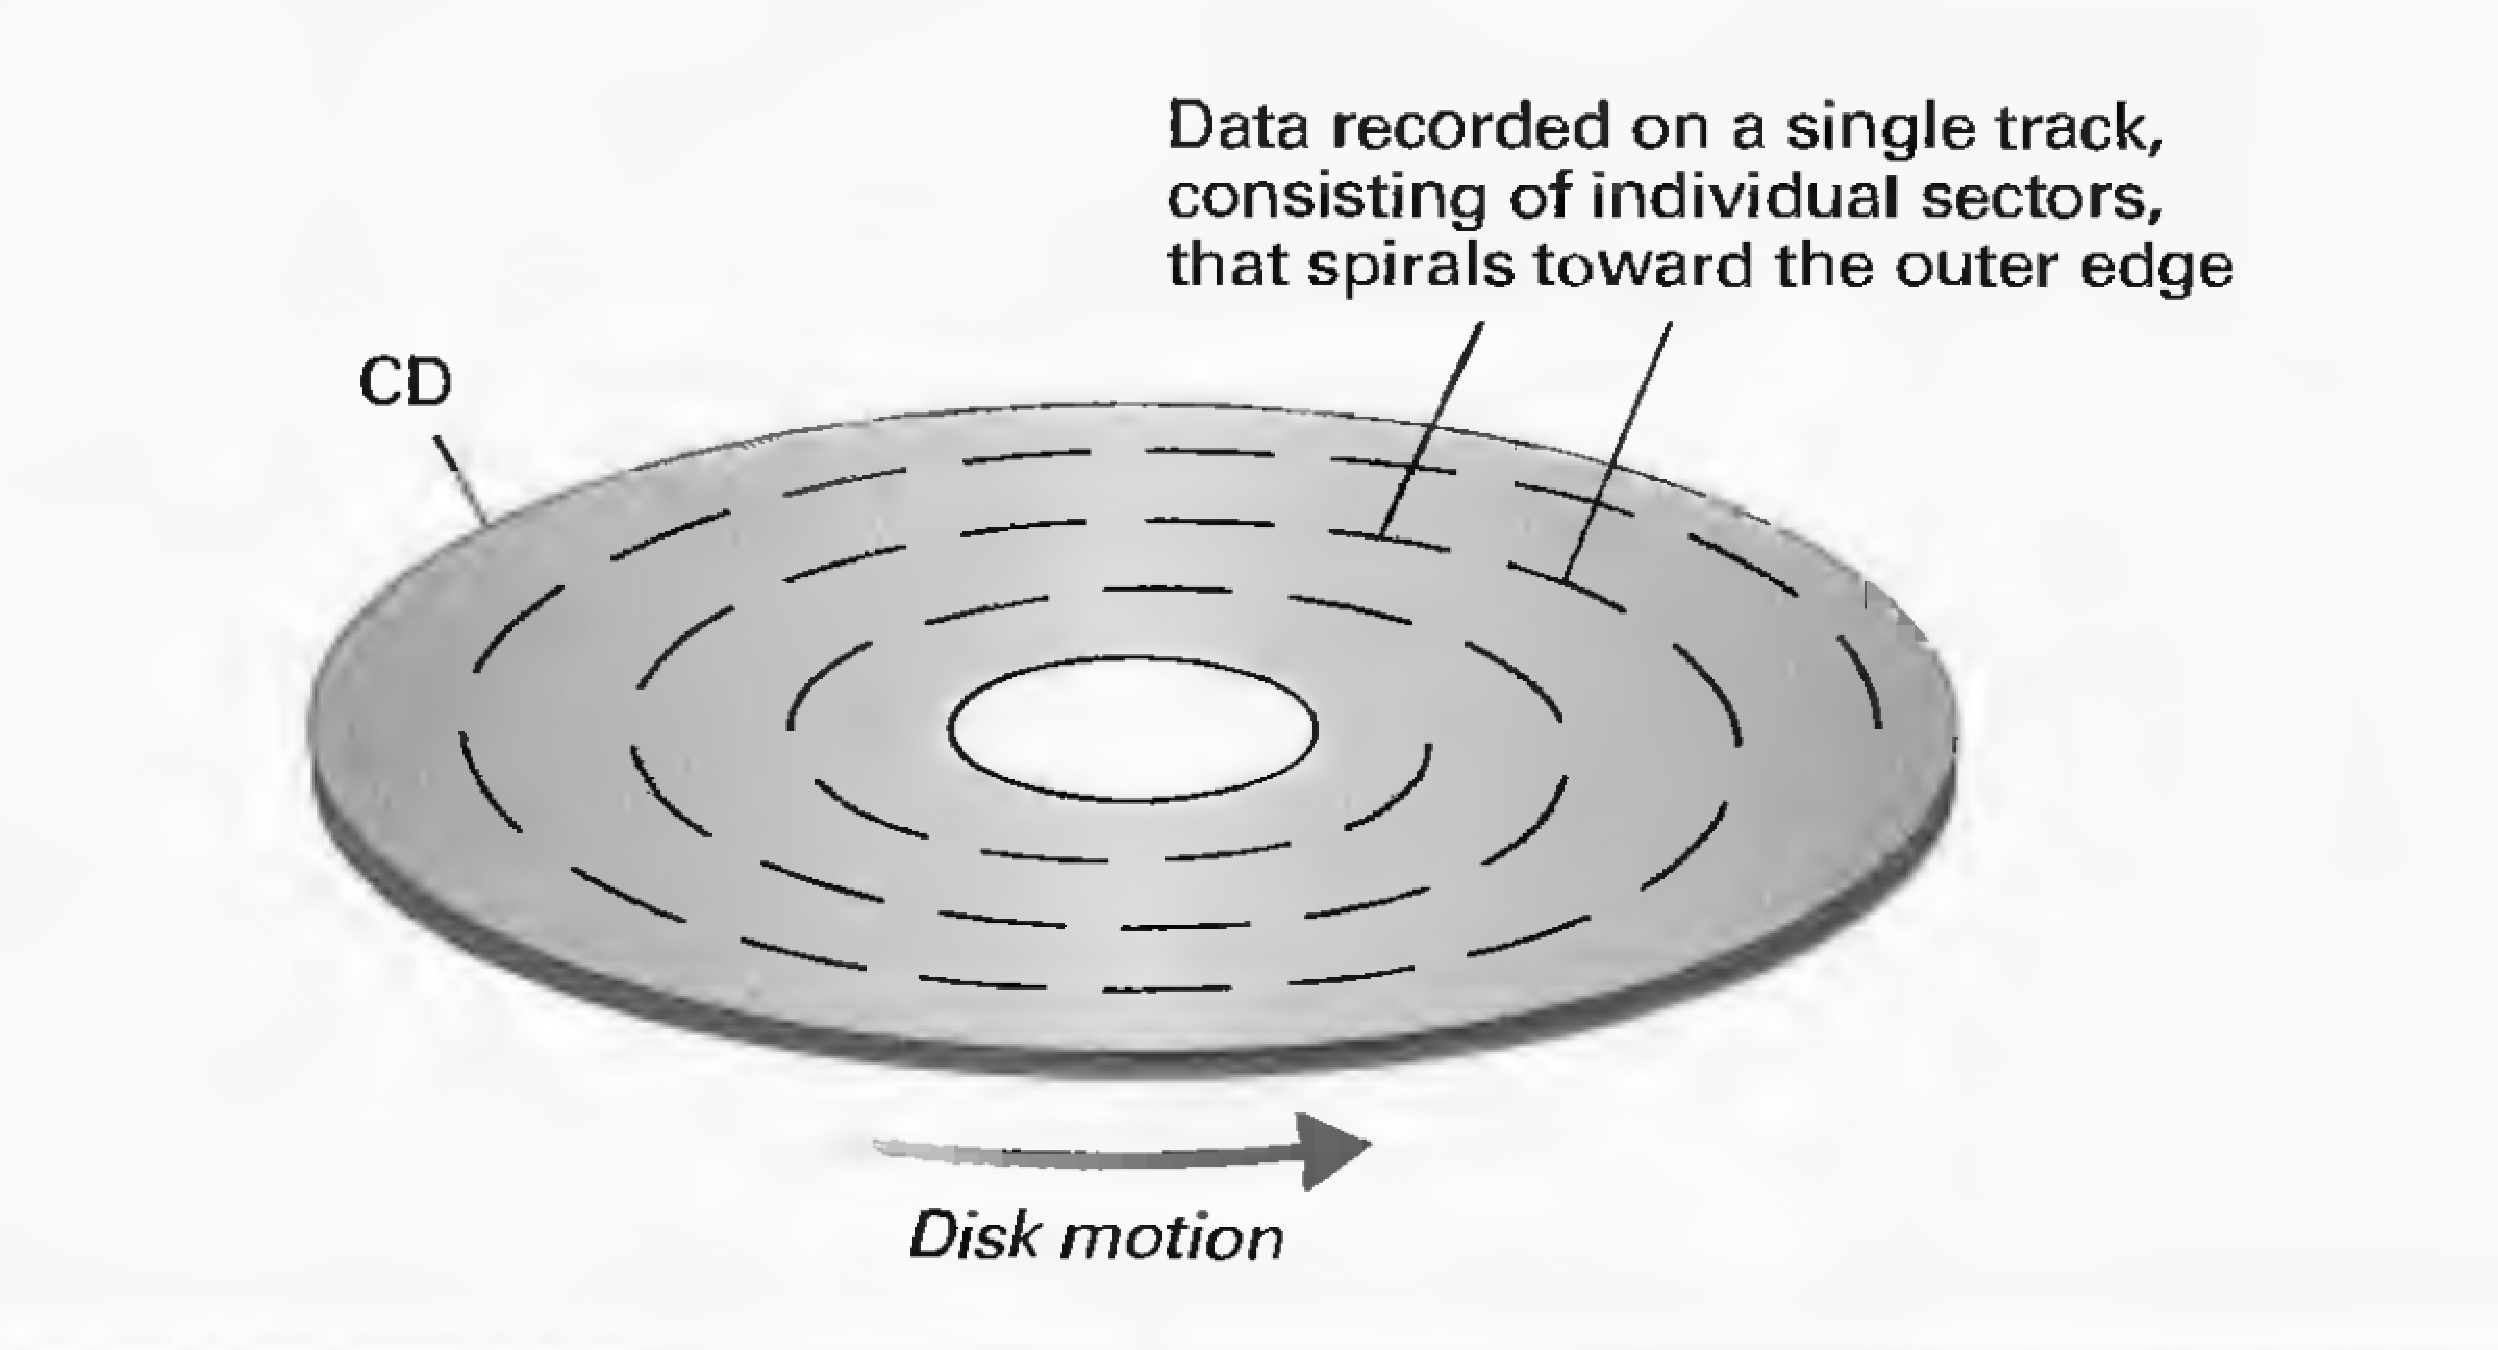
\includegraphics{ch2/Fig1-11.pdf}}
\caption{Định dạng lưu trữ của CD}
  \label{fig:fig1.11}
\end{figure}


% Chú ý rằng khoảng cách quanh track xoắn ốc là lớn dần từ trong ra
% ngoài. Để có thể có khả năng tốt nhất của một CD, các thông tin được
% lưu trữ theo mật đô phân phối tuyến tính chuẩn trên toàn bộ 

%[....]

Như một hệ quả của cách thiết kế, các hệ thống lưu trữ CD thực hiện tốt nhất với xâu dữ
liệu liên tục, dài, giống như khi sản xuất âm nhạc. Ngược lại, khi ứng dụng yêu cầu truy
cập ngẫu nhiên, cách tiếp cận dùng đĩa từ (gồm các track đồng tâm được chia thành các
sector có thể truy cập riêng biệt) làm tốt hơn cách tiếp cận xoắn ốc được dùng trong CDs.

Các đĩa CD truyền thống có khả năng lưu trữ $600$ đến $700$MB. Tuy nhiên, những đĩa
\textbf{DVD (Digital Versatile Disk)}, được xây dựng từ nhiều mối phức tạp, các tầng nửa
trong suốt phục vụ như bề mặt phân biệt khi được nhìn bởi một tia laser hội tụ một cách
chính xác, cho phép khả năng lưu trữ lên tới vài GB. Kiểu đĩa như thế này có khả năng lưu
trữ trình diễn đa phương tiện dài, bao gồm cả hình ảnh chuyển động.

\subsection*{Thiết bị Flash}

Một tính chất chung của thiết bị lưu trữ khối dựa trên công nghệ từ hoặc quang là chuyển
động vật lý như các đĩa xoay, di chuyển đầu đọc, và bắn chùm tia laser, được yêu cầu để
lưu trữ và lấy dữ liệu. Điều này có nghĩa rằng việc lưu trữ dữ liệu và tìm kiếm là chậm so
với mạch điện tử. Công nghệ \textbf{bộ nhớ flash} có khả năng giúp giảm bớt hạn chế
này. Trong hệ thống nhớ flash, các bít được lưu trữ bằng cách gửi tín hiệu điện trực tiếp
tới môi trường lưu trữ ở đó các electron được giữ trong một khoang nhỏ chứa silicon
dioxide, bởi vậy nó biến đổi các đặc trưng của mạch điện. Bởi vì các khoang chứa này có
khả năng giữ các electron trong nhiều năm, nên công nghệ này có thể phù hợp cho việc lưu
trữ dữ liệu off-line.

Mặc dù dữ liệu được lưu trữ trong hệ thống bộ nhớ flash có thể được truy cập theo đơn vị
kích thước nhỏ tính theo byte giống như trong ứng dụng RAM, nhưng hạn chế của công nghệ
hiện nay khiến cho dữ liệu phải được lưu trữ xoá theo khối lớn. Hơn nữa lặp lại việc xoá
sẽ gây thiệt hại cho khoang chứa silicon dioxide. Hạn chế này làm cho công nghệ bộ nhớ
flash hiện tại không thích hợp cho các ứng dụng bộ nhớ chính, nơi yêu cầu nội dung phải
thay đổi nhiều lần trong một giây. Tuy nhiên, đối với các ứng dụng mà tính thay đổi có thể
được điều chỉnh ở mức độ hợp lý như camera số, điện thoại di động, máy PDA cầm tay, thì bộ
nhớ flash lại trở thành thiết bị lưu trữ khối được lựa chọn. Thật vậy, bởi vì bộ nhớ flash
không nhạy cảm với các va chạm về mặt vật lý (ngược lại với hệ thống từ và quang) nên tiềm
năng của nó với các ứng dụng di động là rất hấp dẫn.

Các thiết bị flash được gọi là \textbf{flash drives}, với khả năng lên tới vài GB, là sẵn
có cho các ứng dụng lưu trữ khối tổng quát. Các đơn vị này được nén trong miếng nhựa nhỏ
có độ dài xấp xỉ ba inche cùng với nắp bảo vệ đơn vị kết nối điện khi thiết bị
off-line. Khả năng cao của các đơn vị di động này cũng như sự kiện rằng chúng dễ kết nối
và ngắt kết nối từ máy tính làm cho chúng trở thành lý tưởng cho việc lưu trữ dữ liệu
off-line. Tuy nhiên, tính dễ tổn thương của khoang lưu trữ làm cho chúng không tin cậy như
đĩa quang cho việc lưu trữ thực sự lâu dài.

\subsection*{Lưu trữ và tìm kiếm file}

Thông tin được lưu trữ trong hệ thống lưu trữ khối về mặt thiết kế được nhóm lại thành các
đơn vị lớn gọi là \textbf{file}. Một file điển hình có thể là một tài liệu văn bản được
hoàn thành, một tấm ảnh, một chương trình, một đĩa nhạc, hoặc một tập dữ liệu về nhân viên
trong công ty. Ta đã thấy rằng thiết bị lưu trữ khối làm cho các file được lưu trữ ít
hơn. Ví dụ, một file được lưu trữ trên một đĩa từ phải được xử lý theo sector, mà mỗi
sector có kích thước xác định trước. Một khối dữ liệu phù hợp với đặc trưng của thiết bị
lưu trữ được gọi là \textbf{bản ghi vật lý}. Bởi vậy, một file lớn được lưu trữ trong
thiết bị lưu trữ khối nói chung sẽ bao gồm nhiều bản ghi vật lý.

Ngược lại với cách chia theo các bản ghi vật lý này, một file thường phân chia tự nhiên
theo thông tin được biểu diễn. Ví dụ, một file chứa thông tin về nhân viên trong một công
ty có thể bao gồm nhiều đơn vị, mỗi đơn vị chứa thông tin về một nhân viên. Hoặc một file
chứa tài liệu văn bản có thể bao gồm nhiều đoạn hoặc trang văn bản. Các khối dữ liệu xuất
hiện tự nhiên như thế này được gọi là \textbf{các bản ghi logic}.


Các bản ghi logic thường bao gồm các đơn vị nhỏ hơn gọi là các \textbf{trường}. Ví dụ, một
bản ghi logic chứa thông tin về nhân viên có thể bao gồm trường tên, địa chỉ, số chứng
minh của nhân viên,... Đôi khi mỗi bản ghi logic trong một file xác định một cách duy nhất
bởi một trường đặc biệt bên trong bản ghi (có thể là số chứng minh thư của nhân viên, một
số, hoặc chỉ mục trong bảng liệt kê). Trường xác định như thế này được gọi là
\textbf{trường khoá}. Giá trị giữa trong trường khoá được gọi là \textbf{khoá}.
\begin{figure}
\centering
    \scalebox{0.3}{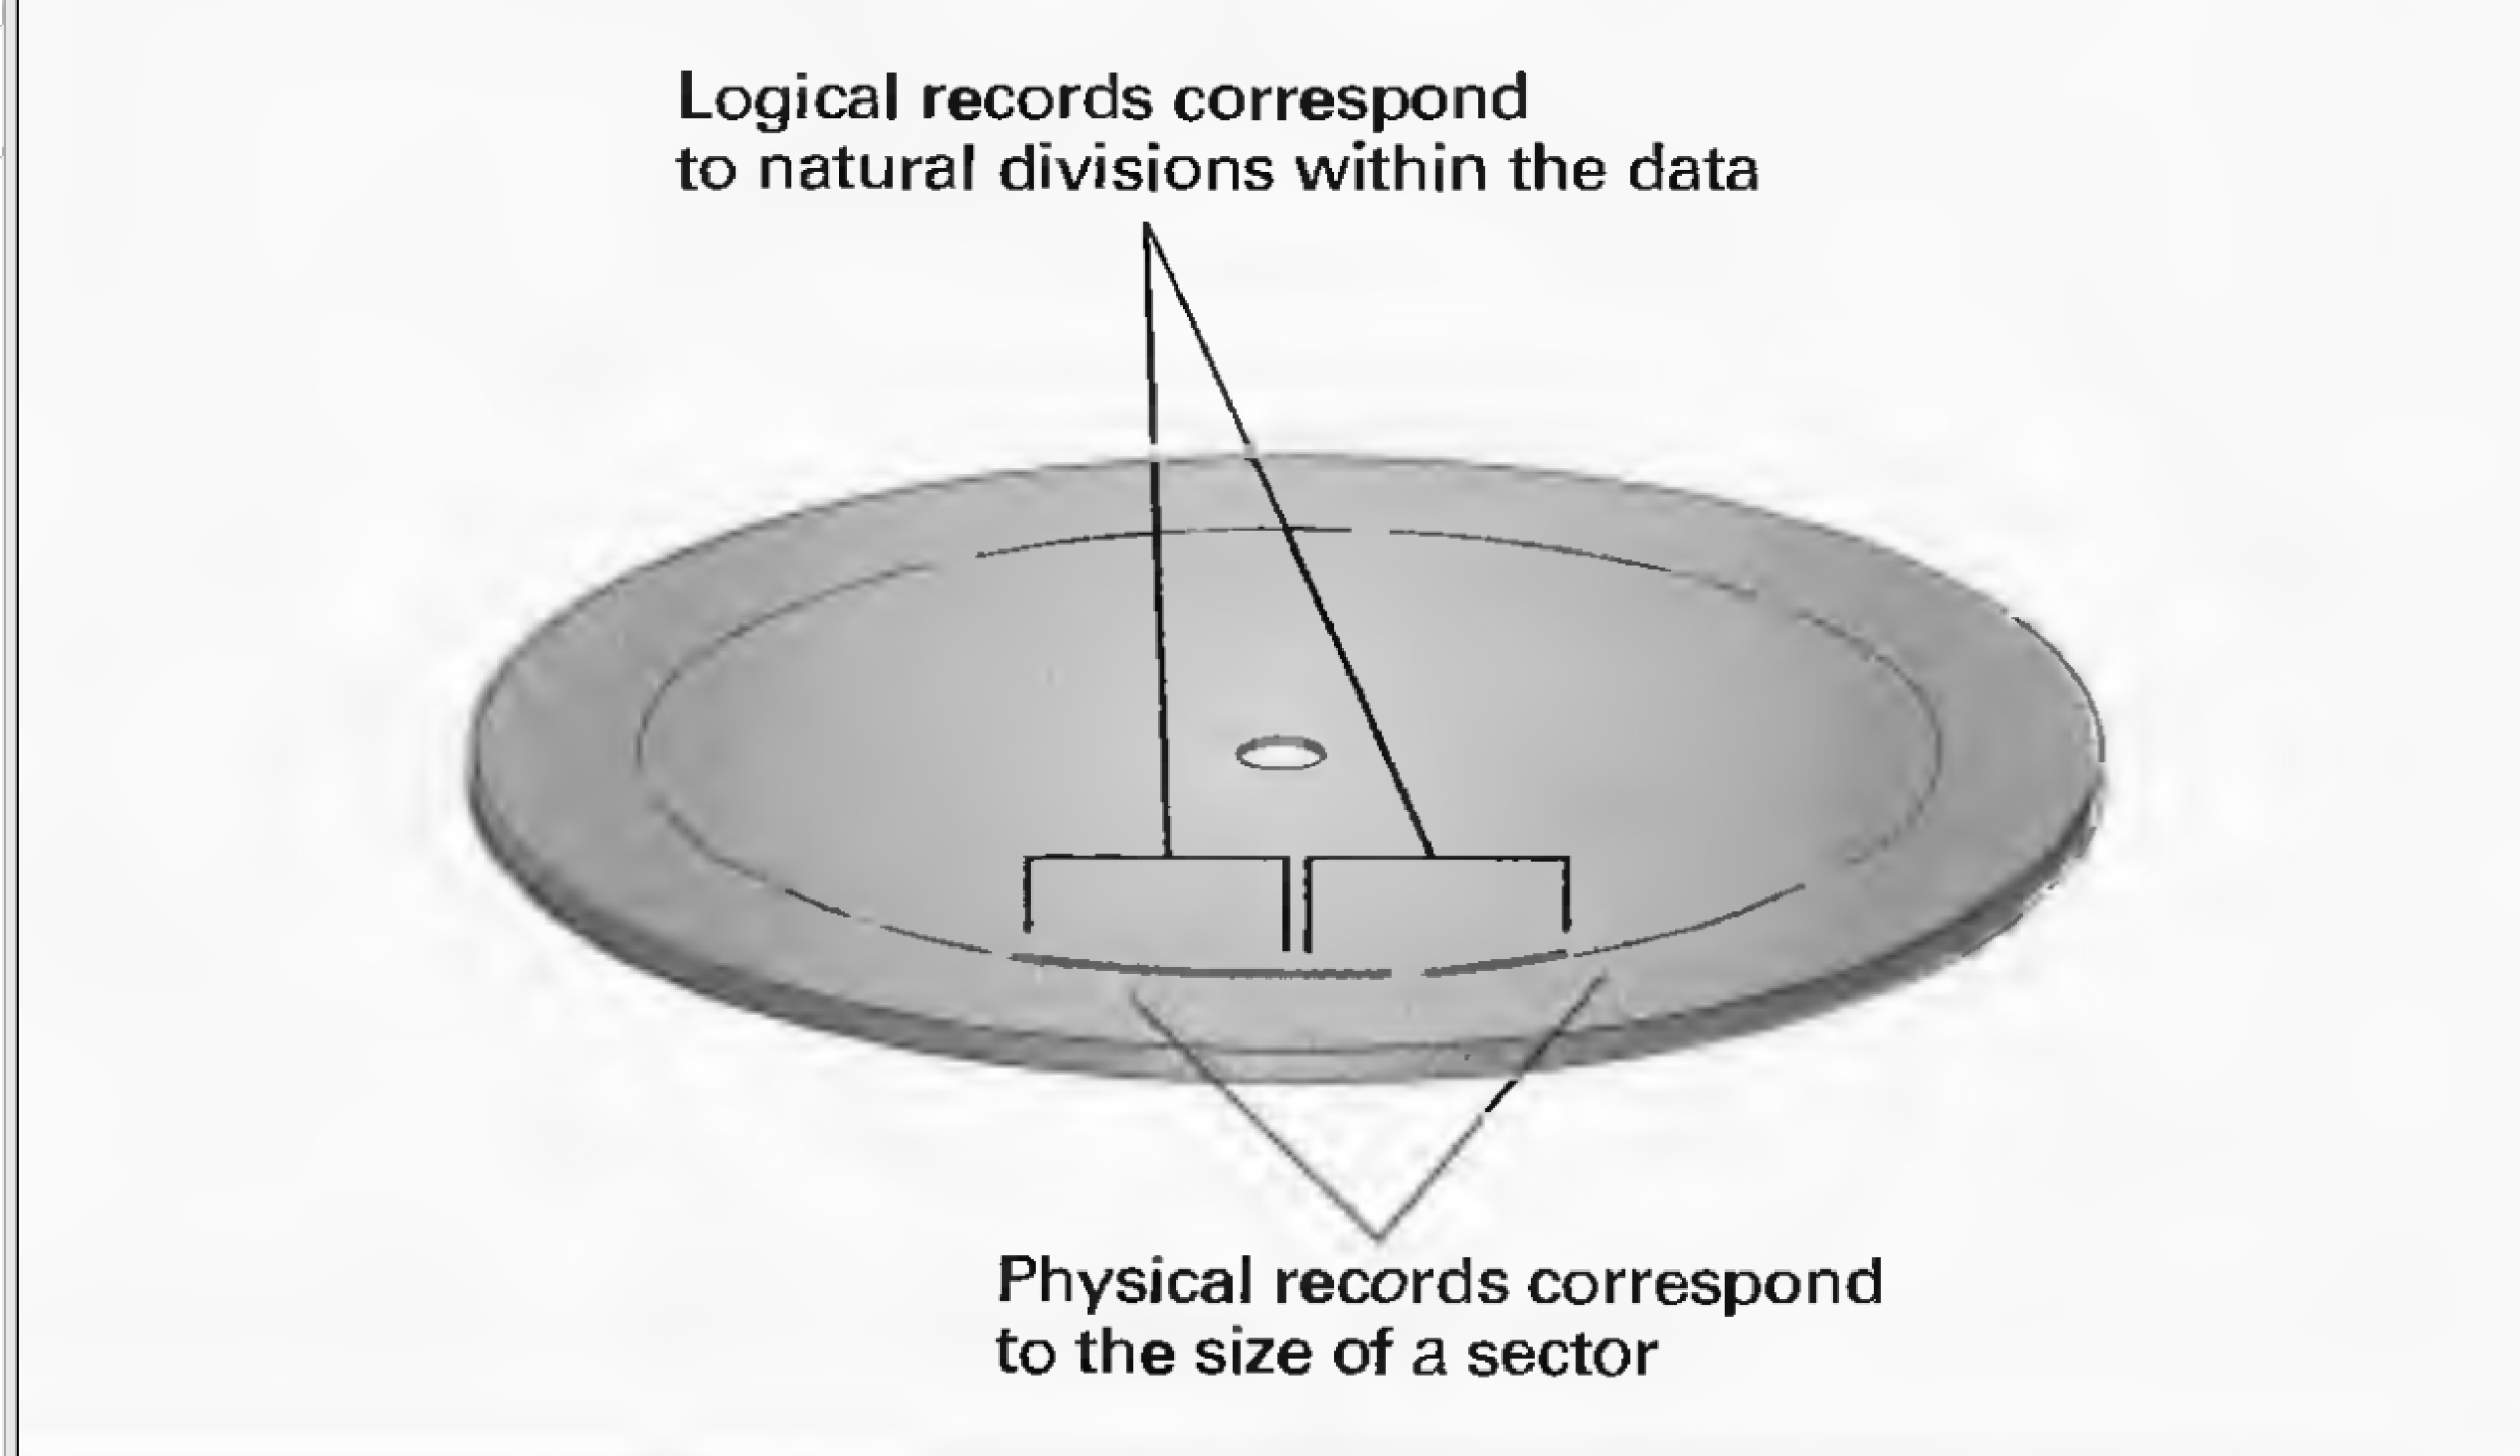
\includegraphics{ch2/Fig1-12.pdf}}
\caption{Bản ghi logic và bản ghi vật lý trên một đĩa}
  \label{fig:fig1.12}
\end{figure}

Các kích thước của bản ghi logic hiếm khi được so sánh với kích thước bản ghi vật lý của
của thiết bị lưu trữ khối. Nói cách khác, người ta có thể tìm thấy một vài bản ghi logic
nằm bên trong một bản ghi vật lý hoặc có thể là một bản ghi logic tách thành hai hoặc
nhiều bản ghi vật lý (Hình \ref{fig:fig1.12}). Kết quả là việc tìm kiếm dữ liệu từ thiết
bị lưu trữ khối phải kèm thêm với việc phục hồi những lộn xộn này. Một giải pháp chung cho
vấn đề này là đặt bên ngoài bộ nhớ chính khoảng đủ lớn lưu giữa một vài bản ghi vật lý và
để sử dụng không gian bộ nhớ này như một vùng nhóm lại. Có nghĩa rằng, các khối dữ liệu
thích hợp với bản ghi vật lý có thể được truyền giữa bộ nhớ chính và thiết bị lưu trữ
khối, trong khi dữ liệu nằm trong bộ nhớ chính có thể được tham khảo như bản ghi logic.


Một vùng bộ nhớ dùng theo cách này được gọi là \textbf{vùng đệm} (buffer). Nói chung, một
vùng đệm là một vùng nhớ được dùng để lưu trữ dữ liệu trung gian trong quá trình truyền dữ
liệu từ thiết bị này tới thiết bị khác. Ví dụ, các máy in hiện đại có chứa mạch nhớ riêng,
phần lớn của mạch này được dùng như vùng đệm để lưu trữ các phần của tài liệu còn chưa
được in mà máy in nhận được.
  
\subsection*{Câu hỏi \& Bài tập}

\begin{enumerate}
\item Hệ thống đĩa cứng có ưu điểm gì so với đĩa mềm khi các đĩa của nó quay nhanh hơn các
  đĩa của đĩa mềm?

\item Khi ghi dữ liệu trên hệ thống nhiều đĩa, ta nên hoàn thành hết bề mặt đĩa trước khi
  bắt đầu bề mặt khác, hay ta đầu tiên nên hoàn thành hết cylinder trước khi bắt đầu sang
  cylinder khác?

\item Trong một hệ thống đặt chỗ, dữ liệu thường phải cập nhật liên tục. Tại sao dữ liệu
  này nên được lưu trữ trên đĩa từ thay vì CD hay DVD?

\item Khi sửa một tài liệu với trình xử lý văn bản, đôi khi việc thêm đoạn văn bản không
  làm tăng kích thước bên ngoài của file trong lưu trữ khối. Nhưng có lúc chỉ thêm một kí
  tự cũng có thể làm tăng kích thước của file tới vài nghìn byte. Bạn hãy giải thích xem
  tại sao?

\item Nêu một vài ưu điểm của thiết bị flash so với hệ thống lưu trữ khác được giới thiệu
  trong phần này?


\item Vùng đệm là gì?
  
\end{enumerate}


  

%%% Local Variables: 
%%% mode: latex
%%% TeX-master: "../tindaicuong"
%%% End: 
